% Created 2021-12-18 sáb 02:30
% Intended LaTeX compiler: pdflatex
\documentclass{article}
\usepackage[utf8]{inputenc}
\usepackage[T1]{fontenc}
\usepackage{graphicx}
\usepackage{grffile}
\usepackage{longtable}
\usepackage{wrapfig}
\usepackage{rotating}
\usepackage[normalem]{ulem}
\usepackage{amsmath}
\usepackage{textcomp}
\usepackage{amssymb}
\usepackage{capt-of}
\usepackage{hyperref}
\usepackage[spanish]{babel}
\usepackage{pifont}
\usepackage{cancel}
\usepackage{pagecolor,lipsum}
\usepackage{svg}
\setcounter{secnumdepth}{2}
\author{Luis Eduardo Galindo Amaya}
\date{\today}
\title{Cálculo Multivariable}
\hypersetup{
 pdfauthor={Luis Eduardo Galindo Amaya},
 pdftitle={Cálculo Multivariable},
 pdfkeywords={},
 pdfsubject={},
 pdfcreator={Emacs 26.3 (Org mode 9.1.9)}, 
 pdflang={Spanish}}
\begin{document}

\maketitle
\tableofcontents


\section{Preámbulo}
\label{sec:org38793cc}
Este es un trabajo en proceso, todavía no ha sido finalizado y todavía no ha sido revisado. Sí tienes alguna idea para alguna corrección puedes mandarme un correo a mi correo \href{mailto:egalindo54@uabc.edu.mx}{egalindo54@uabc.edu.mx}.

\subsection{Sistema Algebraico Computacional}
\label{sec:orgfb15835}
Estos apuntes están hechos para usarse en conjunto con el software CAS de George Weigt, Eigenmath, intentaré pasar los apuntes a Maxima en el futuro por si algo llegara a pasar.

\subsection{Especificaciones}
\label{sec:org46ac76b}
\begin{itemize}
\item Todos los ángulos son en radianes.
\item Utilizaré la notación de subíndices al derivar, por ejemplo \(F_x\) es derivada de la variable 'x' y \(F_{xy}\) es la derivada de 'x' y luego la derivada de 'y'.
\item Cuando escriba un vector emplearé la notación \vec{A}, prefiero emplear las negritas a modo de énfasis.
\item Los diagramas que aparecen aquí son meramente orientativos, por lo tanto, pueden o pueden no representar los nombres de las variables que empleo para las explicaciones.
\end{itemize}

\section{Interpretar un plano}
\label{sec:org109eab9}
\subsection{Eje coordenado}
\label{sec:org9f88870}
Un eje coordenado es una sección en la que dividimos una región del plano para después numerarla, usualmente los llamamos 'x', 'y' y 'z'.

\subsection{Cuadrante}
\label{sec:orgbc508e1}
En Geometría euclidiana plana recibe el nombre de cuadrante cada una de las cuatro regiones infinitas en que los ejes del Sistema Cartesiano bidimensional dividen al plano. Estos cuadrantes están numerados de 1 al 4 (empezando en el superior derecho, en sentido anti-reloj) y denotados por números Romanos.

\subsection{Octante}
\label{sec:org2fd4040}
Un octante en geometría del espacio es cada una de las ocho divisiones coordenadas cartesianas tridimensionales dividen al espacio euclidiano definido por los signos de las coordenadas. Es similar al cuadrante bidimensional y al semi eje mono-dimensional.

\begin{figure}[htbp]
\centering
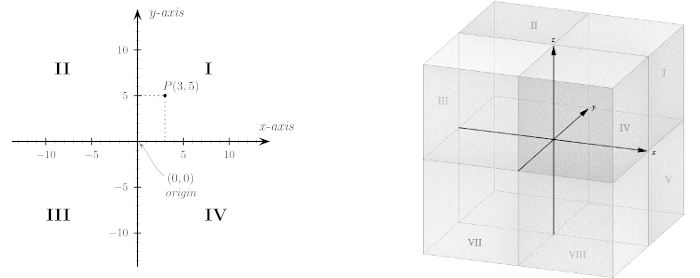
\includegraphics[width=250px]{img/cuadrante-y-octante-2.png}
\caption{A la derecha cuadrantes y a la izquierda los octantes.}
\end{figure}

\section{Representación De Punto En El Plano}
\label{sec:org0ea12f9}
Cuando trabajamos con planos cartesianos podemos marcar puntos indicando el número de su coordenada en cada respectivo eje, está una forma muy rápida de interpretar un punto en el espacio, sin embargo, no es la única y sobre todo cuando trabajamos con funciones circulares las representaciones rectangulares terminan complicando nuestro trabajo.

\subsection{Rectangular o Cartesianas}
\label{sec:orgfb02ed5}
Las coordenadas rectangulares son las coordenadas con las que hemos trabajado todo este tiempo, se representa con un número en cada eje coordenado y para extenderlo simplemente agregamos un número extra para cada valor que deseamos representar. 

\begin{figure}[htbp]
\centering
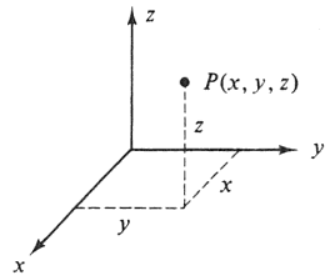
\includegraphics[width=4cm]{img/coordenadas-cartesianas.png}
\caption{Coordenadas Rectangulares.}
\end{figure}

\subsection{Polar o Cilíndrica}
\label{sec:orgdbffddf}
Una coordenada polar tiene dos partes principales, una longitud o radio (r) y un ángulo (\(\theta\)), como cabe imaginar podemos representar figuras circulares con mucha facilidad, también es la notación más común para vectores en física.

\begin{figure}[htbp]
\centering
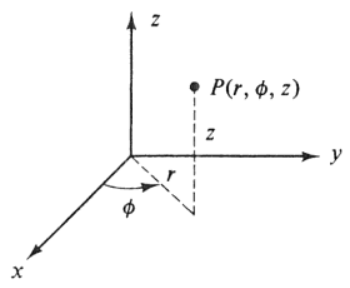
\includegraphics[width=4cm]{img/coordenadas-cilindricas.png}
\caption{Coordenadas Cilíndricas.}
\end{figure}

Podemos extender esta representación en el espacio añadiendo el eje 'z', el cual nos indicara la altura hacia donde apunta el vector.

\subsection{Esférica}
\label{sec:orgc5c7b67}
La representación esférica solo existe en el espacio, y como lo indica su nombre solo representa un valor en un volumen esférico, esta representación utiliza un radio que abarca los tres ejes (\(\rho\) \footnote{Esta letra se lee como rho, no confundir con p.}) dos ángulos para indicar la dirección del punto que deseamos representar, uno para los ejes 'x' y 'y' (\(\theta\)) y uno para el eje 'z' (\(\phi\)).

\begin{figure}[htbp]
\centering
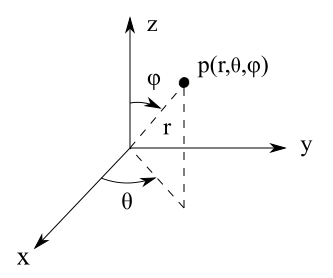
\includegraphics[width=4cm]{img/coordenadas-esfericas.png}
\caption{Coordenadas esféricas.}
\end{figure}


\section{Conversión Entre Sistemas De Coordenadas}
\label{sec:org54a551d}
Ocasionalmente, tenemos que hacer conversiones entre dos o más sistemas de coordenadas, para hacer estas conversiones es necesario tomar en cuenta las propiedades geométricas de cada sistema.

\subsection{Rectangulares A Polares}
\label{sec:orgb4df810}
Las Coordenadas polares están compuestas de dos partes, un radio y un ángulo, tenemos dos fórmulas para calcular cada uno de los componentes: 

\[\begin{aligned}
 r = \sqrt{x^2+y^2} && \theta = arctg\left(y/x\right) \\
\end{aligned}\] 

\textbf{Importante:} Estamos despejando un triángulo y dependiendo el cuadrante donde se encuentre el punto tenemos que sumar los ángulos que nos faltan: 

\begin{center}
\label{tab:orgeeb347f}
\begin{tabular}{|c|c|c|c|}
\hline
Cuadrante & Grados & Radianes\\
\hline
I & 0° & 0\\
II & 180° & \(\pi\)\\
III & 180° & \(\pi\)\\
IV & 360° & 2\(\pi\)\\
\hline
\end{tabular}
\end{center}

\subsection{Rectangulares A Cilíndricas}
\label{sec:org32d22e5}
las coordenadas cilíndricas son una extensión al espacio de las coordenadas polares, por lo tanto, solo convertimos las coordenadas de los ejes 'x' y 'y' a polares y añadimos el eje de las 'z' sin hacer ningún cambio.

\subsection{Rectangulares A Esféricas}
\label{sec:orgb96932c}
Las coordenadas cilíndricas son otra forma de representar las coordenadas polares en el espacio, pero a comparación de las coordenadas cilíndricas ahora usamos dos ángulos para representar la dirección hacia la que apunta el vector: 

\[\begin{aligned}
 \rho = \sqrt{x^2+y^2+z^2} && 
 \theta = arctg\left( y/x \right)  &&
 \phi = arccos\left( z/\rho \right) \\
\end{aligned}\] 

\begin{itemize}
\item \textbf{Importante}
\begin{enumerate}
\item El ángulo \(\phi\) (phi) \textbf{NO} necesita corrección.
\item El ángulo \(\theta\) (theta) \textbf{Si} ocupa \hyperref[tab:orgeeb347f]{corrección}.
\end{enumerate}
\end{itemize}

\subsection{Polares A Rectangulares}
\label{sec:org9afe997}
La conversión de polares a rectangulares se puede hacer directamente con las siguientes fórmulas: 

\[\begin{aligned}
 x = r \cos(\theta) && y = r \sin(\theta) \\
\end{aligned}\] 

Cada una corresponde a un eje coordenado, recordemos que las coordenadas polares únicamente sirven para representar puntos en el plano, por lo tanto, si queremos representar puntos en el espacio tendremos que usar coordenadas cilíndricas.

\subsection{Polares A Cilíndricas}
\label{sec:org2090a97}
Las coordenadas cilíndricas son la extensión directa de las coordenadas polares en el espacio, por lo tanto, tendremos que tomar el valor rectangular de nuestra coordenada en el eje 'z' y añadirla a nuestra representación polar.

\subsection{Cilíndricas A Rectangulares}
\label{sec:org7a6921b}
Para esta conversión simplemente tenemos que hacer las siguientes sustituciones:

\[\begin{aligned}
 x = r \cos(\theta) && y = r \sin(\theta) && z = z \\
\end{aligned}\] 

\subsection{Cilíndricas A Esféricas}
\label{sec:orgb3fbcae}
Para hacer esta conversión es necesario extender el radio a tres dimensiones y calcular el ángulo faltante, como ya tenemos el ángulo \(\theta\) (theta) no tenemos que hacer correcciones al ángulo.

\[\begin{aligned}
 \rho = \sqrt{r^2+z^2} && 
 \theta = \theta  &&
 \phi = arccos\left( z/\rho \right) \\
\end{aligned}\] 

\subsection{Esféricas A Rectangulares}
\label{sec:org5259651}
Para esta conversión simplemente tenemos que hacer las siguientes sustituciones:

\[\begin{aligned}
 x = \rho \sin(\phi)\cos(\theta) && 
 y = \rho \sin(\phi)\sin(\theta) &&
 z = \rho \cos(\phi) \\
\end{aligned}\] 

\subsection{Esféricas A Cilíndricas}
\label{sec:orga9db68e}
para convertir las coordenadas esféricas a cilíndricas tendremos que convertir el ángulo \(\phi\) (phi) a su coordenada cartesiana 'z':

\[\begin{aligned}
 r = \rho \sin(\phi) && 
 \theta = \theta &&
 z = \rho \cos(\phi) \\
\end{aligned}\] 

\section{Vectores}
\label{sec:org660867d}
Un vector es la representación matemática y gráfica de una magnitud vectorial. Consiste básicamente en una flecha o segmento rectilíneo orientado, es decir, con una determinada longitud, dirección y sentido, y que contiene toda la información de la magnitud que se está midiendo. Ejemplos de vectores: 

\[\begin{aligned}
  (x,y,z) && (r,\theta) && (\rho, \theta, \phi) \\
\end{aligned}\] 

\subsection{Representación}
\label{sec:org9d51026}
En física usualmente se representan los vectores de forma polar ó cilíndrica, con una magnitud y un ángulo, pero esto no tiene por que ser siempre así, en calculo multivariable con mucha frecuencia se utiliza la la notación cartesiana (tres números dentro de un paréntesis representando cada eje coordenado) ó también la compleja (donde cada uno componentes es una variable 'i' es x 'j' es 'y' y 'z' es 'k'), ejemplo el vector (1,3,4) se puede representar de manera compleja como el punto 'i + 3j + 4k'. 

\subsection{Notación}
\label{sec:org6651091}
Para identificar que un valor es un vector hay dos formas principales añadiendo una flecha en la parte superior de la variable (\(\vec{A}\)) o resaltando el nombre de la variable con negritas. 

\subsection{Vector Negativo}
\label{sec:orgc64f6fa}
Si un vector tiene el símbolo negativo, todos sus componentes cambian su signo: 

\[
-\vec{A} = (-\vec{A_1},-\vec{A_2},...,-\vec{A_n})
\]

\uline{Esto si el vector está en coordenadas rectangulares}, cuando el vector está en polar añadimos 180° grados al ángulo: 

\[ \begin{aligned}
\vec{A} = (3,75^\circ) && -\vec{A} = (3,-75^\circ) = (3,255^\circ)
\end{aligned} \]

\subsection{Suma y Resta de Vectores}
\label{sec:org087b763}
Sumar vectores no representa más que la suma de independiente de cada uno de sus componentes.

\[
\vec{A} + \vec{B} = (\vec{A}_x + \vec{B}_x,\vec{A}_y + \vec{B}_y,\vec{A}_z + \vec{B}_z)
\]

\[
\vec{A} - \vec{B} = (\vec{A}_x - \vec{B}_x,\vec{A}_y - \vec{B}_y,\vec{A}_z - \vec{B}_z)
\]

\textbf{Importante:} Esto es solo para coordenadas cartesianas, si tenemos nuestro vector en coordenadas cilíndricas o esféricas tendremos que hacer la conversión correspondiente.

\subsection{Multiplicación Escalar}
\label{sec:org1ef6df1}
Podemos multiplicar un vector por un valor fijo para aumentar su tamaño, simplemente multiplicamos cada componente por la constante de nuestro interés:

\[
k \cdot \vec{A} = (k\cdot\vec{A_x},k\cdot\vec{A_y},k\cdot\vec{A_z})
\]

\subsection{Módulo o magnitud del Vector}
\label{sec:org8d6c01a}
El módulo de un vector es la longitud entre el inicio y el final del vector, podemos calcular la distancia desde el origen con la fórmula de distancia:

\[
\vert\vec{A}\vert = \sqrt{ x^2 + y^2 + z^2 }
\]

\subsubsection*{Módulo del Vector Fuera Del Origen}
\label{sec:orgb98565a}
Hay ocasiones en las que tenemos un vector que no parte desde el origen de nuestra gráfica, para eso simplemente tenemos que restar al vector el punto de origen, por ejemplo sí tenemos un vector \(\vec{A} = (3,5,6)\) con origen en \(g = (5,6,3)\) simplemente las restamos:

\[ \begin{aligned}
\vec{A} &= (3-5,5-6,6-3) \\
~ &= (-2,-1,3) \\
\end{aligned} \]

De este modo podemos calcular la magnitud del vector independientemente de su origen:

\[ \begin{aligned}
\vec{A} &= (-2,-1,3) \\
\vert\vec{A}\vert &= \sqrt{14} \\
\end{aligned} \]

\subsection{Producto Punto}
\label{sec:org56a8a1e}
Para representar el producto punto usamos el operador \(\cdot\). Al producto punto también se le llama comúnmente producto escalar, ya que el resultado \uline{siempre es una escalar}. Es producto punto en palabras sencillas es la suma de la multiplicación componente por componente:

\[
\vec{A} \cdot \vec{B} = \vec{A}\vec{B}^T
\]

\[
\vec{A} \cdot \vec{B} = \vec{A}_1 \vec{B}_1 + \vec{A}_2 \vec{B}_2 + ... + \vec{A}_n \vec{B}_n
\]

Una propiedad muy importante que debemos tener en cuenta es su relación con los ángulos de los vectores, esto es muy útil para determinar los ángulos directores más adelante:

\[
 \vec{A}\cdot\vec{B} = \vert\vec{A}\vert\vert\vec{B}\vert \cos(\theta)
\]

\subsection{Producto Cruz}
\label{sec:org4f8801f}
El producto cruz al igual que el producto punto representa una operación que raciona dos vectores y sus magnitudes, su operador es \(\times\), a comparación del producto punto el resultado \uline{No es un escalar}, el producto cruz siempre devuelve otro vector:

\[
\vec{A} \times \vec{B} = \det\begin{pmatrix}
       i    &      j    &     k    \\
  \vec{A_x} & \vec{A_y} & \vec{A_z}\\
  \vec{B_x} & \vec{B_y} & \vec{B_z}\\
\end{pmatrix}
\] 

\[
\vec{A} \times \vec{B} = 
  (\vec{A_y}\vec{B_z} - \vec{A_z}\vec{A_y})i + 
  (\vec{A_z}\vec{B_x} - \vec{A_x}\vec{A_z})j + 
  (\vec{A_x}\vec{B_y} - \vec{A_y}\vec{A_x})k
\]

Al igual que el producto punto el producto cruz representa la relación geométrica, la fórmula es muy parecida más, sin embargo, ahora usamos el seno en vez del coseno, entre dos vectores:

\[
\vert \vec{A}\times\vec{B}\vert = \vert\vec{A}\vert\vert\vec{B}\vert \sin(\theta)
\]

\subsection{Producto Mixto}
\label{sec:org2387fc6}
Se le conoce también como triple producto escalar, es la operación que combina el producto punto y el producto cruz\footnote{El resultado es un escalar.}:

\[
\vec{A}\cdot(\vec{B}\times\vec{C}) = \det\begin{pmatrix}
  \vec{A_x} & \vec{A_y} & \vec{A_z}\\
  \vec{B_x} & \vec{B_y} & \vec{B_z}\\
  \vec{C_x} & \vec{C_y} & \vec{C_z}\\
\end{pmatrix}
\]

\section{Aplicaciones De Vectores}
\label{sec:org3372b88}
\subsection{Vector Unitario}
\label{sec:orga39017d}
La característica fundamental del vector unitario es que su longitud siempre es igual a '1', no importa la dirección o el cuadrante mientras el módulo es igual a '1' entonces es unitario. El vector unitario es muy útil para determinar la dirección de un vector sin tener que tomar en cuenta su magnitud. Para calcularlo simplemente dividimos los valores de nuestro vector entre el módulo.

\[ 
\hat{A} = \frac{\vec{A}}{\vert\vec{A}\vert} 
\]

\subsection{Ángulos Entre Vectores}
\label{sec:org48bb6f4}
Si recordamos una de las propiedades del producto punto y el producto cruz es que representan la relación entre el ángulo y las magnitudes de los vectores:

\[ \begin{aligned}
 \vec{A}\cdot\vec{B} = |\vec{A}||\vec{B}| \cos(\theta) && |\vec{A}\times\vec{B}| = |\vec{A}||\vec{B}| \sin(\theta) \\
\end{aligned} \]

Entonces si despejamos los vectores obtenemos las siguientes fórmulas:

\[ \begin{aligned}
\cos(\theta) = \frac{\vec{A} \cdot \vec{B}}{|\vec{A}||\vec{B}|} &&
\sin(\theta) = \frac{|\vec{A}\times\vec{B}|}{|\vec{A}||\vec{B}|} \\
\end{aligned} \]

\subsection{Ángulos Directores}
\label{sec:org708ef1f}
Es aquel ángulo entre un vector y uno de los ejes (ya sea 'x', 'y' o 'z'), para calcularlo solo tenemos que medir el ángulo entre nuestro vector y el eje que nos interesa conocer:

\[\begin{aligned}
  \cos(\alpha) = \frac{a_x}{|\vec{a}|} &&
  \cos(\beta)  = \frac{a_y}{|\vec{a}|} &&
  \cos(\gamma) = \frac{a_z}{|\vec{a}|} \\
\end{aligned} \]

\begin{figure}[htbp]
\centering
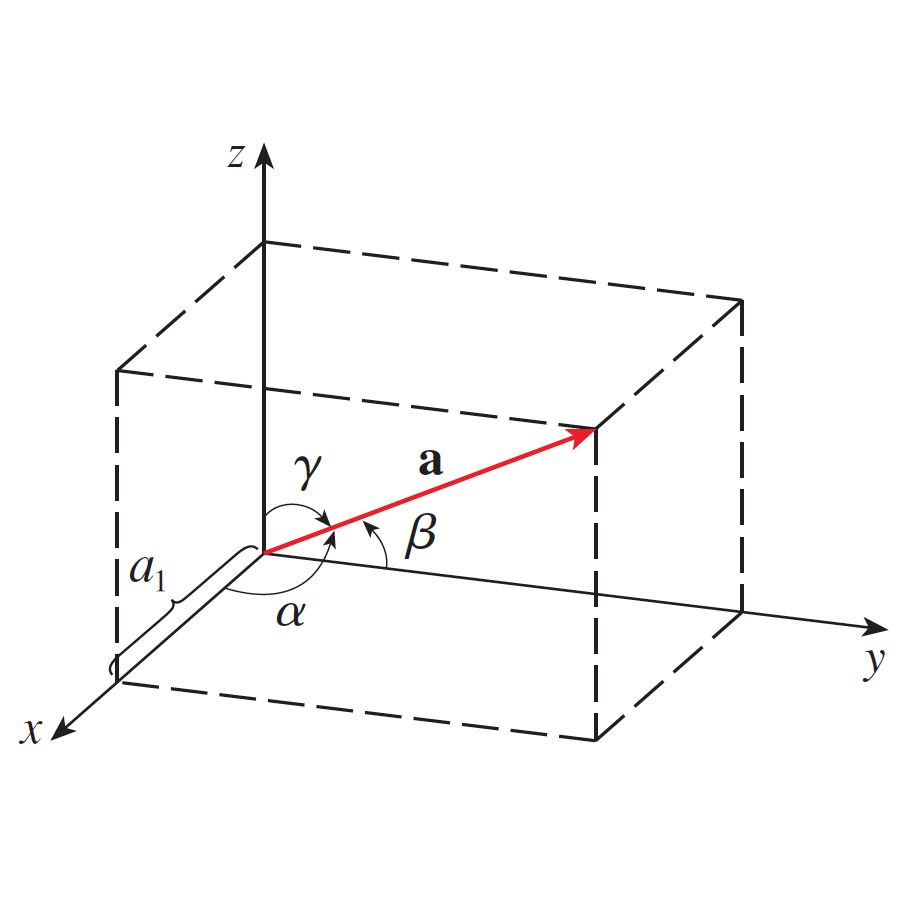
\includegraphics[width=4cm]{img/angulos-directores.png}
\caption{Ángulos directores de \(\vec{a}\).}
\end{figure}


\subsubsection*{Despeje Del Los Ángulos Directores:}
\label{sec:orga5163b8}
Estas fórmulas se despejan de la fórmula del producto punto, como es un vector unitario el eje los valores que no usamos se anulan automáticamente\footnote{También es posible usar el producto cruz para este procedimiento, pero por simplicidad se prefiere el producto punto.}:

\[\begin{aligned}
  cos(\alpha) &= \frac{a_x \cdot 1 + \cancel{a_y \cdot 0~} + \cancel{a_z \cdot 0} }{|\vec{a}| \cdot \sqrt{1^2+\cancel{0^2}+\cancel{0^2}}} \\
  cos(\alpha) &= \frac{a_x \cdot 1}{|\vec{a}| \cdot 1} \\
  cos(\alpha) &= \frac{a_x}{|\vec{a}|} \\
\end{aligned} \]

\subsection{Área De Un Paralelogramo}
\label{sec:org2993ea2}
Si tenemos dos vectores podemos calcular el área del paralelogramo que se forma simplemente usando el producto cruz, Esto lo podemos verificar son el siguiente diagrama:

\begin{figure}[htbp]
\centering
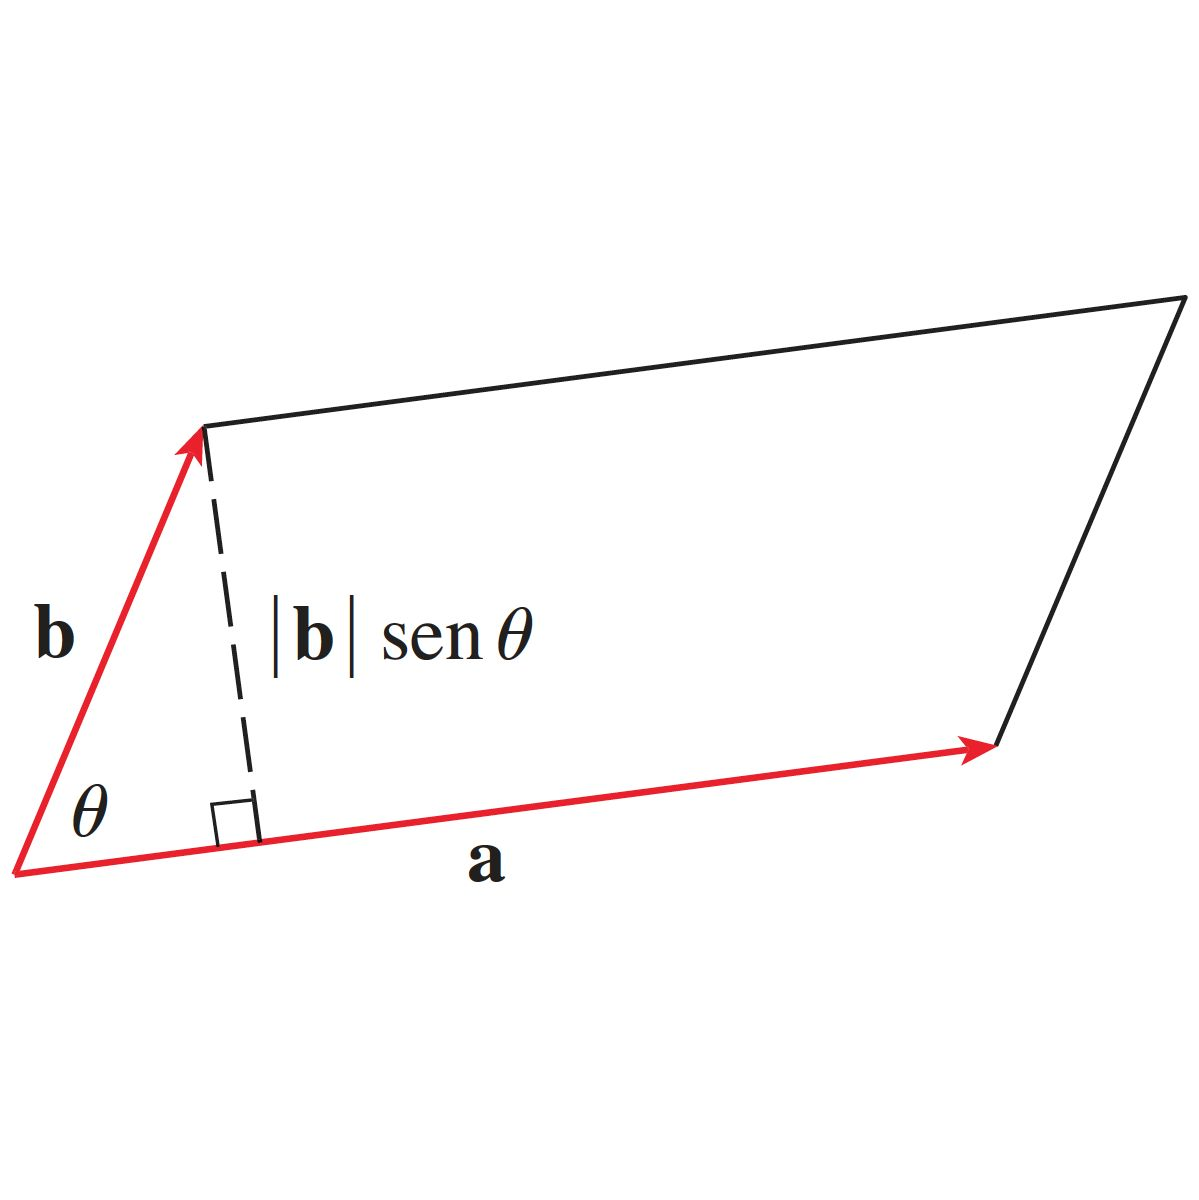
\includegraphics[width=4cm]{img/producto-cruz.png}
\caption{Paralelogramo.}
\end{figure}

En primaria aprendimos que el área del paralelogramo es base por altura, sin embargo, la altura del paralelogramo no se puede obtener midiendo sus lados, ya que está inclinado, si aplicamos trigonometría podemos saber que el valor del cateto opuesto (la altura) es igual al seno del ángulo, entonces la fórmula quedaría:

\[
  {\text{Área} = \text{base} \cdot \sin(\theta)}
\]

Y esto es exactamente al valor del \uline{producto cruz de dos vectores}:

\[
  {|a \times b|=|a||b|\sin(\theta)}
\]

\subsection{Área Del Triángulo}
\label{sec:org1f51da5}
Sabemos que el área del triángulo es igual al área de un rectángulo entre '2' también sabemos que el área del paralelogramo es su producto cruz, entonces para encontrar el área solo basta con divir el producto cruz entre '2':

\begin{center}
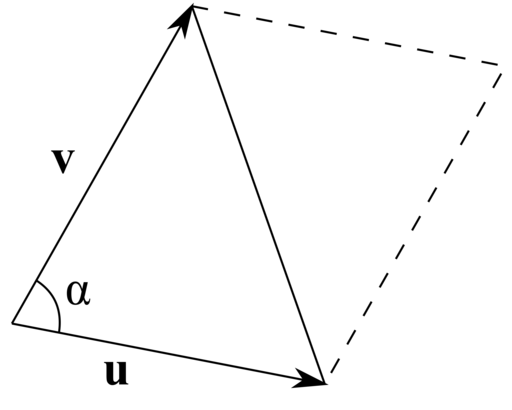
\includegraphics[width=3cm]{img/area-triangulo.png}
\end{center}

\[
A = \frac{1}{2}|\vec{u}\times\vec{v}|
\]

\subsection{Volumen De Un Paralelepípedo}
\label{sec:org623d12e}
Si queremos extender el paralelogramo a R\(^{\text{3}}\) obtendremos un paralelepípedo que, al igual que el paralelogramo, podemos formarlo simplemente con vectores y como conocemos sus propiedades es fácil determinar su volumen aplicando el producto mixto:

\begin{center}
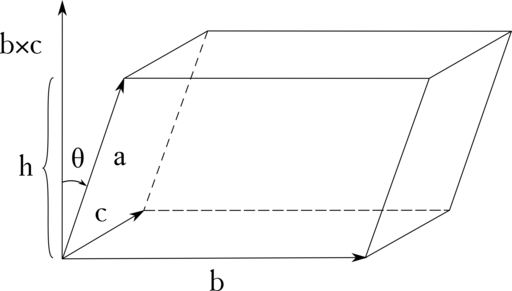
\includegraphics[width=4cm]{img/paralelipedo.png}
\end{center}

\[
V = \vec{a}\cdot(\vec{b}\times\vec{c}) = \det\begin{pmatrix}
  a_x & a_y & a_z \\
  b_x & b_y & b_z \\
  c_x & c_y & c_z \\
\end{pmatrix}
\]

\subsection{Volumen De Un Tetraedro}
\label{sec:orge3d78a2}
Al igual que con el paralelepípedo el tetraedro es una forma de extender una figura del plano al espacio, en este caso el triángulo, el volumen del tetraedro es igual a una sexta parte del producto mixto:

\[
V = \frac{1}{6} \left( \vec{a}\cdot\left[\vec{b}\times\vec{c}\right] \right)
\]

\subsection{Determinar Sí Dos Vectores Son Ortogonales}
\label{sec:org9914e91}
Dos vectores son ortogonales (perpendiculares), si su producto escalar equivale a cero.

\[
\vec{A} \cdot \vec{B} = 0
\]

\section{Parametrización De Curvas Planas}
\label{sec:org8783ab0}
La parametrización es una forma que tenemos en matemáticas de representar una función en con una tercera variable 't' de la cual dependen 'x' y 'y'.

\subsection{Parametrización De Una Recta}
\label{sec:org86ca9f1}
Una de las ventajas que tenernos con la parametrización es que podemos definir una función si conocemos algunos de los puntos, por ejemplo si queremos parametrizar una recta de la cual desconocemos su función, pero de la cual tenemos dos puntos podemos usar la siguiente fórmula:

\[
P_0 + t(p_1 - p_0)
\]

en donde 'P\(_{\text{0}}\)' y 'P\(_{\text{1}}\)' son los puntos que conocemos y 't' es una variable continua, Ejemplo si tenemos los puntos \(P_0 = <1,2>\) y \(P_1 = <3,4>\) sustituimos en la fórmula:

\[ \begin{aligned} f(t) &= \begin{cases}
  x: 1 + t (3-1) \\
  y: 2 + t (4-2) \\
\end{cases} \\ &= \begin{cases}
  x: 1 + 2t \\
  y: 2 + 2t \\ 
\end{cases} \end{aligned} \]

Una de las cosas que tenemos que notar es como tenemos una función para cada eje coordenado\footnote{La fórmula anterior se puede extender a R\(^{\text{3}}\).}, si lo graficamos notaremos que si 't' es igual a '0' el valor que obtendremos es igual a P\(_{\text{0}}\), pero si el valor de 't' es '1' el valor que obtenemos será igual a P\(_{\text{1}}\).

\subsection{Curvas Planas Más Comunes}
\label{sec:orgf4d8e9d}
\begin{longtable}{|c|c|c|c|}
\hline
Nombre & Parametrizacion & Ecuación & Rango\\
\hline
\endfirsthead
\multicolumn{4}{l}{Continúa de la página anterior} \\
\hline

Nombre & Parametrizacion & Ecuación & Rango \\

\hline
\endhead
\hline\multicolumn{4}{r}{Continúa en la siguiente página} \\
\endfoot
\endlastfoot
\hline
 &  &  & \\
 & \((^x_y)=P_0(1-t)+P_1t\) &  & \\
Recta &  & \(y-y_1=m(x-x_1)\) & \(0\leq t\leq 1\)\\
 & \((^x_y)=P_0+t(P_1-P_0)\) &  & \\
 &  &  & \\
\hline
 &  &  & \\
Elipse & \((^x_y)=(^{x_1}_{y_1})+\left(^{a\cos t}_{b\sin t}\right)\) & \(\frac{(x-x_1)^2}{a^2}+\frac{(y-y_1)^2}{b^2}=1\) & \(0\leq t\leq 2\pi\)\\
 &  &  & \\
\hline
 &  &  & \\
Parábola & \((^x_y)=(^{x_1}_{y_1})+\left(^{t}_{t^2}\right)\) & \(y-y_1=m(x-x_1)^2\) & ---\\
 &  &  & \\
\hline
 &  &  & \\
Hipérbola & \((^x_y)=(^{x_1}_{y_1})+\left(^{a\sec t}_{b\tan t}\right)\) & \(\frac{(x-x_1)^2}{a^2}-\frac{(y-y_1)^2}{b^2}=1\) & \(0\leq t\leq 2\pi\)\\
 &  &  & \\
\hline
 &  &  & \\
Hipérbola & \((^x_y)=(^{x_1}_{y_1})+\left(^{a\cosh t}_{b\sinh t}\right)\) & --- & \(-2\pi\leq t\leq 2\pi\)\\
(una hoja) &  &  & \\
 &  &  & \\
\hline
\end{longtable}

\section{Funciones y funciones De Dos Ó Mas Variables}
\label{sec:orge074f03}
Anterior mente solo hemos trabajado con funciones de una sola variable, las cuales tiene una variable de entrada y otra de salida, las funciones multivariable son similares, pero ahora \uline{toman dos números y retornan solo uno}. 

\[
f(x,y) = x^2 + y^2 - 1
\]

\subsection{Ecuación Del Plano}
\label{sec:orga6a54aa}
Un plano es un objeto ideal que únicamente posee dos dimensiones, y contiene infinitos puntos y rectas; es un concepto fundamental de la geometría junto con el punto y la recta. Cuando se habla de un plano, se está hablando del objeto geométrico que no posee volumen, es decir bidimensional, y que contiene un número infinito de rectas y puntos. 

\[ax+by+cz+d=0\]

\subsection{Recta En El Espacio}
\label{sec:org6329bf0}
Para representar una recta es necesario hacer una ecuación que represente los ejes de nuestro espacio coordenado:

\[
\frac{x-x_0}{a} = \frac{y-y_0}{b} = \frac{z-z_0}{c}
\]

\subsection{Dominio De Una Función}
\label{sec:org0ad983f}
El dominio de la función es el conjunto de valores que se le puede dar a las variables independientes en una función, por ejemplo:

\[
f(x) = \sqrt{2x+4}
\]

sabemos que la función de raíz cuadrada existe para todos los valores que son igual o mayor a '0' (en números reales), entonces el dominio de la función seria\footnote{Ambas formas de expresarlas son correctas.}:

\[ \begin{aligned}
\{x\in\mathbb{R}:2x+4 \geq 0\} &~& \{x\in\mathbb{R}:x \geq -2\}
\end{aligned} \]

Ahora bien, encontrar el dominio cuando tenemos múltiples variables no es muy diferente, pero dependiendo la función tendremos más condiciones, ejemplo:

\[
f(x,y) = \frac{ \sqrt{x+y+1} }{ x-1 }
\]

al igual que en el ejemplo anterior tenemos una raíz, por lo que sabemos que \(x+y+1\geq 0\), pero además tenemos una división, por lo tanto, tampoco la función existe en donde el denominador es '0', como resultado, el dominio seria:

\[
\{ (x,y) \in \mathbb{R}^2: x + y + 1 \geq 0 \land x \not = 1  \}
\]

quizá ver el dominio así es un poco intimidante, así que la voy a explicar parte por parte:

\begin{itemize}
\item \((x,y)\in\mathbb{R}^2\), la funcion existe en (\(\in\)) los numeros reales cuando\ldots{}
\item \(x+y+1 \geq 0\), la suma de \(x+y+1\) es mayor o igual (\(\ge\)) que 0\ldots{}
\item \(\land\), y\ldots{}
\item \(x \not = 1\), x \textbf{NO} es igual a 1.
\end{itemize}

Es recomendable conocer las funciones discontinuas y en donde son discontinuas para encontrar el rango de manera más rápida.

\subsection{Rango De Una Función}
\label{sec:orga42445e}
El Rango ó imagen es el conjunto de números que dependen de la sustitución (tabulación) de los valores que puede tomar 'x' y 'y' en el dominio, en palabras más sencillas es todos los valores que puede retornar la función:

\[
f(x,y) = \sqrt{9-x^2-y^2}
\]

Es recomendable que antes de buscar el rango de la función determinemos el dominio, esto nos permite separar la función en varias funciones más pequeñas de las cuales podemos encontrar el valor máximo:

\[
\{ (x,y) \in \mathbb{R}^2: x^2 + y^2 \leq 9  \}
\]

Como los valores de 'x' y 'y' se están restando\footnote{Al ser cuadrados los valores que obtenemos siempre son positivos.} y la raíz no puede ser menor a '0' entonces determinamos que el \uline{máximo valor máximo} de \(9-x^2-y^2\) es '9' y como la función es raíz \(\sqrt{9}=3\).

Ahora para el \uline{valor mínimo} no hay mucho misterio, la función es raíz y en los reales no hay raíces negativas, entonces el mínimo valor es 0. Entonces el rango quedaría:

\[
\{ f(x,y) \in \mathbb{R}^2: 0 \leq f(x,y) \leq 3  \}
\]

\subsection{Planos Más Comunes}
\label{sec:orgee6095b}
\begin{longtable}{|p{6cm}|p{5.2cm}|}
\hline
Nombre & Ecuación\\
\hline
\endfirsthead
\multicolumn{2}{l}{Continúa de la página anterior} \\
\hline

Nombre & Ecuación \\

\hline
\endhead
\hline\multicolumn{2}{r}{Continúa en la siguiente página} \\
\endfoot
\endlastfoot
\hline
 & \\
Plano & \(ax+by+cz+d=0\)\\
 & \\
\hline
 & \\
Cilindro elíptico & \(x^2+y^2=1\)\\
 & \\
\hline
 & \\
Cilindro hiperbólico & \(x^2-y^2=1\)\\
 & \\
\hline
 & \\
Elipse & \(\frac{x^2}{a^2}+\frac{y^2}{b^2}+\frac{z^2}{c^2}=1\)\\
 & \\
\hline
 & \\
Paraboloide elíptico & \(z=\frac{x^2}{a^2}+\frac{y^2}{b^2}\)\\
 & \\
\hline
 & \\
Paraboloide hiperbólico & \(z=\frac{x^2}{a^2}-\frac{y^2}{b^2}\)\\
 & \\
\hline
 & \\
Hipérbole de una hoja & \(x^2 + y^2 - z^2 = 1\)\\
 & \\
\hline
 & \\
Hipérbole de dos hojas & \(x^2 - y^2 - z^2 = 1\)\\
 & \\
\hline
 & \\
Cono & \(z^2 = x^2 + y^2\)\\
 & \\
\hline
\end{longtable}

\section{Páginas De Consulta Y Recursos Útiles}
\label{sec:org4794084}
\subsection{Calculadoras}
\label{sec:org8fb442d}
\begin{itemize}
\item Calculadora De Cartesianas A Cilíndricas, \url{https://tinyurl.com/y2ljx8fp}
\item Calculadora De Cilíndricas A Esféricas, \url{https://tinyurl.com/y5dzufw9}
\item \href{https://www.wolframalpha.com/widgets/view.jsp?id=537159240ca725f712f6c7437d2f3e0c}{Máximos y mínimos}
\end{itemize}

\subsection{Páginas}
\label{sec:orgd6cf71a}
\begin{itemize}
\item \url{https://es.wikipedia.org/wiki/Cuadrante\_(geometr\%C3\%ADa)}
\item \url{https://es.wikipedia.org/wiki/Octante\_(geometr\%C3\%ADa)}
\item Coordenadas Cilíndricas A Cartesianas, \url{https://tinyurl.com/y3s49cv3}
\item Coordenadas Cilíndricas Y Esféricas, \url{https://tinyurl.com/y3kdl2jc}
\item Coordenadas Cilíndricas Y Esféricas, \url{https://tinyurl.com/yxu823uh}
\item Definición De Vector, \url{https://tinyurl.com/y675y7lb}
\item Producto Mixto, \url{https://tinyurl.com/y5jzwdy2}
\item Ángulos Directores, \url{https://tinyurl.com/yxvvlh7f}
\item Volúmenes Y Área, \url{https://tinyurl.com/y5s4udhp}
\item \href{https://www.gaussianos.com/representar-superficies-en-tres-dimensiones/}{Representar superficies en tres dimensiones}
\item \href{https://www.superprof.es/apuntes/escolar/matematicas/analitica/recta/ecuaciones-de-la-recta-en-el-espacio.html\#tema\_ecuacion-continua-de-la-recta}{Ecuación de la recta en el espacio}
\item \href{https://personales.unican.es/alvareze/CalculoWeb/CalculoII/apuntes/curvasParametricas.pdf}{Parametrización}
\item \href{https://blog.unitips.mx/dominio-y-rango-de-funciones}{Rango de una función}
\end{itemize}

\subsection{Videos}
\label{sec:orgd9eaedb}
\begin{itemize}
\item Producto Punto Por Zach Star, \url{https://tinyurl.com/y2x8dj88}
\end{itemize}
\end{document}
